\newlecture

\setcounter{section}{5}
%\def\textbookchapter{Chapter 10: Derivatives of Multivariable Functions}
\def\coursetopicnumber{II}
\def\topic{Directional Derivatives and the Gradient} % this is the printed title
\def\shorttopic{Directional derivatives, gradient} % short topic
\def\textbookname{Active Calculus} % this is the corresponding textbook
\def\shorttextbookname{AC} % this is the short name for the book
\def\textbooksection{10.6} % corresponding textbook section
\def\textbooksectionurl{https://activecalculus.org/vector/S-10-6-Directional-Derivative.html} % URL for textbook section
\def\handoutday{} % this is the printed date

%%%%%%%%% DOCUMENT CONTENT STARTS BELOW

\thispagestyle{plain}
\topstuff
\section{\topic{} \booklink{}}
\label{sec:directional-derivative-gradient}
\subsection{Directional derivatives}
For a function $f(x,y)$, thus far we have seen limit definitions for $f_x(x,y)$ and $f_y(x,y)$:
\[
    f_x(x,y)=\lim\limits_{\Delta x\to 0}\dfrac{f(x+\Delta x,y)-f(x,y)}{\Delta x}\quad \text{ and } \quad f_y(x,y)=\lim\limits_{\Delta y\to 0}\dfrac{f(x,y+\Delta y)-f(x,y)}{\Delta y}.
\] 
Our interpretation thus far is that if we are at a point $(a,b)$ in the $xy$-plane, and we move 
\begin{itemize}
    \item eastward (in the positive $x$-direction), then the rate of increase of $f(x,y)$ is 
    \item northward (in the positive $y$-direction), then the rate of increase of $f(x,y)$ is 
\end{itemize}
It turns out that if we know the rate of change of $f$ in these two directions, then we can compute the rate of change of $f$ in ANY direction!

\medskip 

Let $\vec{u}=\langle u_1,u_2\rangle$ be a unit vector that points in the direction we want to move. Suppose we are at the point $P=(a,b)$ and move a distance $h$ in the direction of $\vec{u}$. Our new point $Q$ has coordinates $Q=(a+hu_1,b+hu_2)$. The slope of the secant line connecting these points is 
\[
    \dfrac{\text{rise}}{\text{run}} =     \dfrac{f(Q)-f(P)}{|h\vec{u}|}\hspace{4in}\mbox{}
\]
%\dfrac{f(a+hu_1,b+hu_2)-f(a,b)}{|h\vec{u}|}.\] 
\vspace{1in}

If we let $h$ to go 0, this will give us the slope of the tangent line in the direction of $\vec{u}$ at the point $(a,b)$. In other words, we get the instantaneous rate of change of $f(x,y)$ at $(a,b)$ in the direction $\vec{u}$.
\begin{defn}[Directional Derivative]
    Let $f$ be differentiable at the point $(a,b)$, and let $\vec{u}=\langle u_1,u_2\rangle$ be a unit vector. The \emph{directional derivative of $f$ at $(a,b)$ in the direction of $\vec{u}$} is
    \[
        \D_{\vec{u}}f(a,b)=\lim\limits_{h\to 0}\dfrac{f(a+hu_1,b+hu_2)-f(a,b)}{h}.
    \]
\end{defn}\bigskip

\pagebreak 

\subsection{Computing the directional derivative}
Since the above limit is a single-variable $\frac{0}{0}$ form, we apply l'H\^opital's Rule (from Calculus I):

\begin{align*}
    \D_{\vec{u}}f(a,b)
    &\overset{H}{=}\lim\limits_{h\to0}\dfrac{\frac{\dif}{\dif h}f(a+hu_1,b+hu_2)-\frac{\dif}{\dif h}f(a,b)}{\frac{\dif}{\dif h}h} \\ \\ 
    &= \lim\limits_{h\to0}\dfrac{\frac{\dif}{\dif h} f(x,y)-0}{1} \phantom{\quad\text{ for } x=a+hu_1 \text{ and } y=b+hu_2}
    \\ \\ 
    %&=\lim\limits_{h\to0}\dfrac{f_x(a+hu_1,b+hu_2)\cdot u_1 + f_y(a+hu_1,b+hu_2)\cdot u_2}{1}\\ \\
    &= \\ &
\end{align*}
\vspace{.6in}

\begin{thm}
    Let $f$ be differentiable at the point $(a,b)$, and let $\vec{u}=\langle u_1,u_2\rangle$ be a unit vector. The \emph{directional derivative of $f$ at $(a,b)$ in the direction of $\vec{u}$} is \medskip 
    
    \[
        \D_{\vec{u}}f(a,b)=\phantom{\langle f_x(a,b),f_y(a,b)\rangle\dotp\langle u_1,u_2\rangle.}\hspace{2in}
    \]
\end{thm}
\vspace{1in}

\begin{ex}
    Let $f(x,y)=x^2-7y$. At what rate is $f(x,y)$ changing at the point $(1,2)$ if we move in the direction of the vector $\vec{v}=\left\langle 3,-4\right\rangle$?
\end{ex}

\vspace{2in}

\pagebreak

\subsection{The gradient}
\begin{defn}
    Let $f(x,y)$ be differentiable at the point $(x,y)$. The \emph{gradient} of $f$ at $(x,y)$ is the vector-valued function 
    \[
        \nabla f(x,y)=\phantom{\langle f_x(x,y),f_y(x,y)\rangle = f_x(x,y)\vec{i}+f_y(x,y)\vec{j}.}
    \]
\end{defn}

If $f(x,y,z)$ is differentiable at the point $(x,y,z)$, then
\[
    \nabla f(x,y,z)=\phantom{\langle f_x(x,y,z),f_y(x,y,z),f_z(x,y,z)\rangle = f_x(x,y,z)\vec{i}+f_y(x,y,z)\vec{j}+f_z(x,y,z).}
\]
\medskip 

\begin{ex}
    Let $f(x,y)=3xy+\dfrac{x-2y}{x+y}+5$. Compute $\nabla f(x,y)$.
\end{ex}

\vspace{2in}

\begin{ex}
    How are gradients and differentials related?
\end{ex}

\vspace{1in}

Note that we can use a gradient to compute a directional derivative! For $\vec{u}$ a unit vector, since $\nabla f(x,y)=\langle f_x(x,y),f_y(x,y)\rangle$, \[\D_{\vec{u}} f(a,b) = \hspace{2in}\]% \nabla f(a,b)\dotp \vec{u}.\]
\medskip 

More generally, if $\vec{v}$ is any nonzero vector, then the directional derivative of $f(x,y)$ at $(a,b)$ in the direction of $\vec{v}$ is \[\D_{\vec{v}} f(a,b) = \hspace{2in}\]
\pagebreak 
\begin{ex}
    Consider the surface defined by $z=f(x,y)=x^2+5y^2$. Here is a sketch of its level curves for $c = 0, 5, 10, 15, 20, 25, 30, 35$. The point $P=(5,-1)$ is also marked.
    \bigskip 
    
    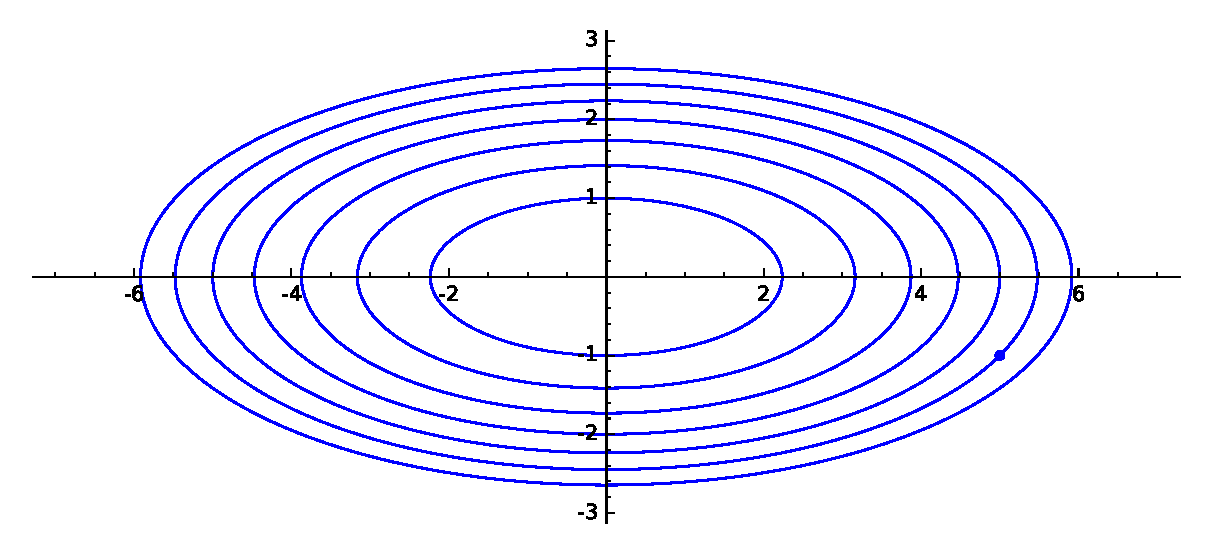
\includegraphics[width=.7\textwidth]{images/circles.eps}\label{img:sage-level-curves-again}
    \begin{enumerate}
        %\item Name the surface.
        \item Sketch the surface.
        \item Find the equation of the level curve through the point $P=(5,-1)$.
        \item Let $\vec{v}_1=\langle 2,-3\rangle$, $\vec{v}_2=\langle 1,1\rangle$, $\vec{v}_3=\langle -1,0\rangle$. 
        Decide if the directional derivatives of $f$ at $P$ in the directions $\vec{v}_1$, $\vec{v}_2$, $\vec{v}_3$ are positive, negative, or zero.
        \item Still with $f(x,y)=x^2+5y^2$, compute $\nabla f(x,y)$.
        \item Compute $\D_{\vec{v}_1}f(P)$, $\D_{\vec{v}_2}f(P)$, and $\D_{\vec{v}_3}f(P)$.
    \end{enumerate}
\end{ex}

\pagebreak 

\subsection{The direction and magnitude of the gradient}
We have seen that the directional derivative of $f$ at $(a,b)$ in the direction of a unit vector $\vec{u}$ is 
\[
    \D_{\vec{u}} f(a,b) = \nabla f(a,b)\dotp \vec{u}.
\] 
This tells us the rate at which $f$ changes if we are at the point $(a,b)$ and move in the direction $\vec{u}$.

Since this involves a dot product, we can think of this in terms of the angle $\theta$ between the vectors $\nabla f(a,b)$ and $\vec{u}$:
\begin{align*}
    \D_{\vec{u}}f(a,b) 
    &= \nabla f(a,b)\dotp\vec{u} \hspace{2in} \\ \\
    & = \\ %& = |\nabla f(a,b)|\, |\vec{u}| \cos\theta,\\
    %& = |\nabla f(a,b)| \cos\theta.
\end{align*}

\noindent Then, since $-1\le \cos\theta \le 1$, the directional derivative $\D_{\vec{u}}f(a,b)$
\begin{itemize}
    \item has its maximum value when $\cos\theta=1$, so when $\theta=$ \\  
    \medskip 
    
    \noindent Therefore the maximum value of $\D_{\vec{u}}f(a,b)$ is \\
    \item has its minimum value when $\cos\theta=-1$, so when $\theta=$ \\  
    \medskip 
    
    \noindent Therefore the minimum value of $\D_{\vec{u}}f(a,b)$ is \\
\end{itemize}

Another important value of $\cos\theta$ is 0. When $\cos\theta=0$, we have $\D_{\vec{u}}f(a,b)=$

\bigskip 

The theorem below summarizes these observations.
\vspace{.5in}

\begin{thm}[Directions of change]\label{thm:dirs-of-change}
    Let $f$ be differentiable at $(a,b)$ with $\nabla f(a,b)\ne \vec{0}$.
    \begin{enumerate}
        \item $f$ has its maximum rate of increase at $(a,b)$ in the direction of the gradient $\nabla f(a,b)$. The rate of change in this direction is $|\nabla f(a,b)|$.\\
        \item $f$ has its maximum rate of decrease at $(a,b)$ in the direction of $-\nabla f(a,b)$. The rate of change in this direction is $-|\nabla f(a,b)|$.\\
        \item The directional derivative is zero in any direction orthogonal to $\nabla f(a,b)$.
    \end{enumerate}
\end{thm}


\pagebreak 

\begin{ex}
    Consider the elliptic paraboloid $z=f(x,y)=x^2+y^2$.
    \begin{enumerate}
        \item In the contour diagram below, mark the point $P=(2,-1)$. Label its level curve as well as the two level curves closest to it. (The level curves are $c=0,1,2,\dots,9$.)
        \item If you are on the paraboloid at the point $(x,y,z)=(2,-1,5)$, in which direction in the $xy$-plane should you move in order to \emph{ascend} on the surface at the maximum rate? What is the rate of change? 
        \item If you are on the paraboloid at the point $(2,-1,5)$, in which direction in the $xy$-plane should you move in order to \emph{descend} on the surface at the maximum rate? What is the rate of change? 
        \item At the point $(2,-1,5)$, in what direction(s) in the $xy$-plane is there no change in the value of $f(x,y)$?
    \end{enumerate}
\end{ex}

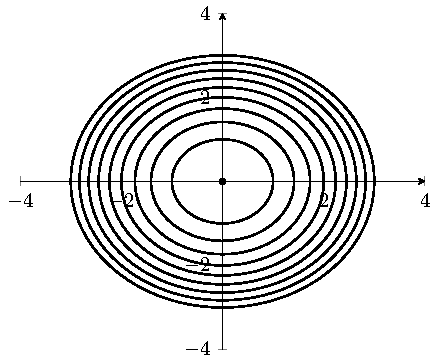
\includegraphics[scale=1]{tikz-pictures/section-9.1-again-pic3-level-curves-elliptic-paraboloid-1.pdf} 
\hfill  
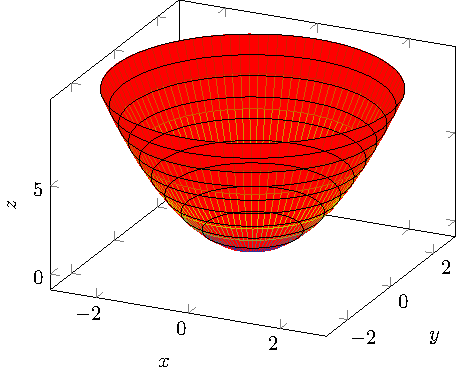
\includegraphics[scale=1]{tikz-pictures/section-9.1-again-pic3-level-curves-elliptic-paraboloid-3.pdf}\label{img:tikz-paraboloid-again}

\pagebreak 
\noindent The third part of Theorem \ref{thm:dirs-of-change} gives us an important relationship between level curves and the gradient.

\begin{thm}
    Given a function $f$ differentiable at $(a,b)$, the line tangent to the level curve of $f$ at $(a,b)$ is orthogonal to the gradient $\nabla f(a,b)$.
\end{thm}
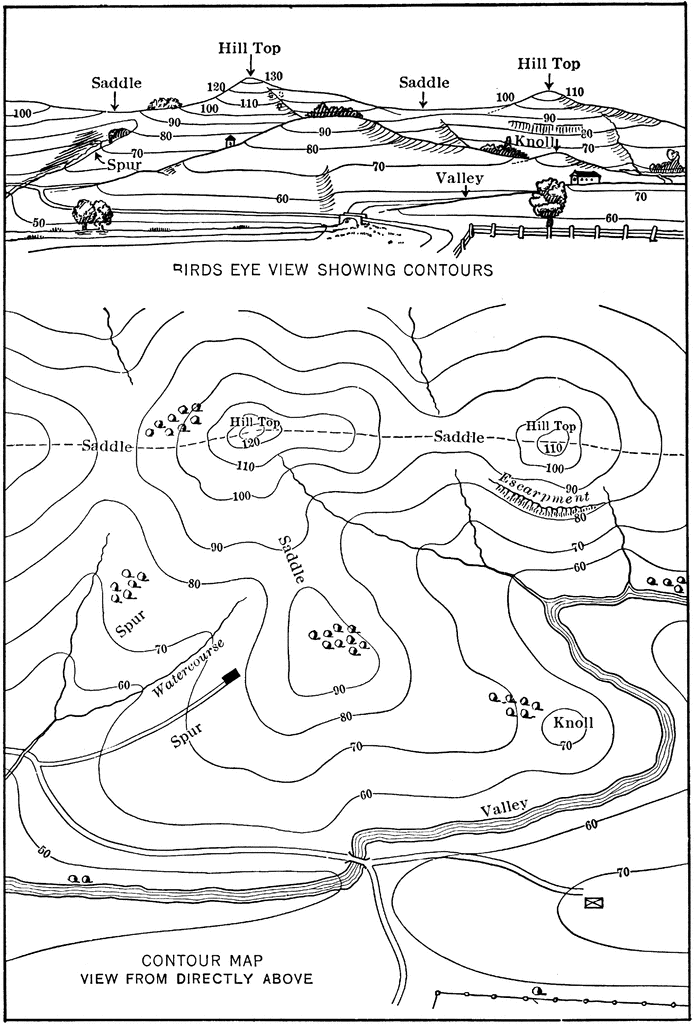
\includegraphics[width=.5\textwidth]{images/contour-map.png}\label{img:fcit-contour-diagram}
\hfill  
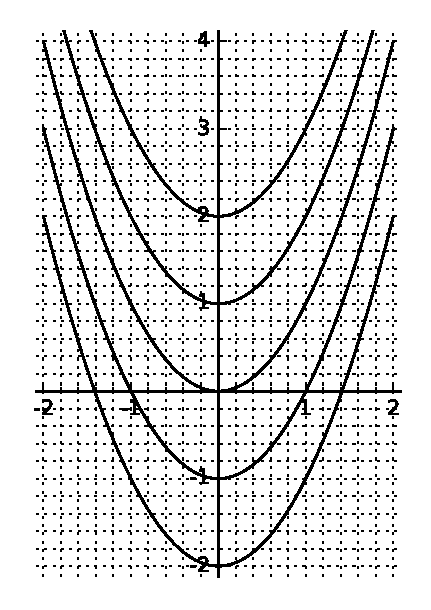
\includegraphics[width=.48\textwidth]{images/parabolas.eps}\label{img:sage-parabolas-gradient}

\begin{ex}
    Let $f(x,y)=y-x^2$. Level curves for $c=-2,-1,0,1,2$ are given above. Determine the direction of and sketch the gradient vector $\nabla f(a,b)$ at the following points: $(0,2)$, $(1,-1)$, $(-1,2)$.
    \vfill\mbox{}
    \let\thefootnote\relax\footnote{Clipart courtesy FCIT, \href{https://etc.usf.edu/clipart/}{\tt https://etc.usf.edu/clipart/}.}
    \addtocounter{footnote}{-1}\let\thefootnote\svthefootnote

\end{ex}

\pagebreak 


